\begin{figure}[ht]
\centering
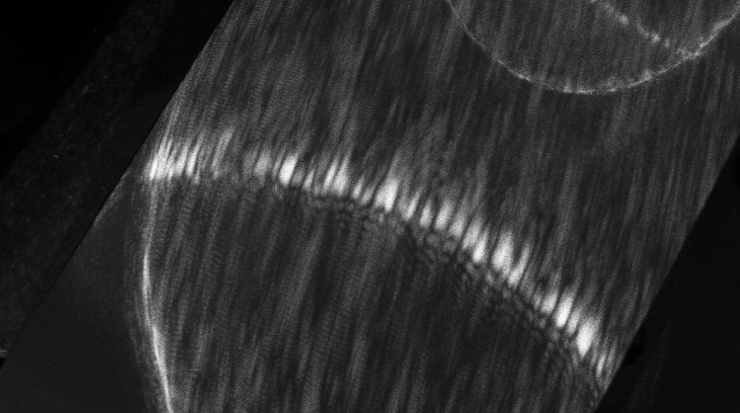
\includegraphics[keepaspectratio,width=15cm]{speckle/figures/Ag_LaSFN9_cone_lens11_cam-8899.jpg}
\caption{A portion of the cone speckle, projected on to a piece of paper.}
\label{fig:examplespeckle}
\end{figure}

Under most circumstances, light scattered in to the cone is not homogeneous
but exhibits distinctive intensity fluctuations known as \textit{speckle}.
In optics, this arises due to the interference of coherent waves with
randomly distributed amplitudes and phases.  Speckle in optics is closely
related to the mesoscopic phenomena of universal conductance
fluctuations~\cite{lee1985universal}, and likewise exhibits many of the
same interesting physics such as coherent
backscattering~\cite{akkermans1986coherent}.  This chapter is devoted to
our studies of speckle in the cone.  Here we examine the properties of cone
speckle and compare them with traditional systems.  We also discuss certain
features and correlations which are useful in the context of biosensing.
